\documentclass{article}
\usepackage[utf8]{inputenc}
\usepackage{geometry}
\usepackage{polski}
\usepackage{float}
\usepackage{graphicx}
\usepackage[shortlabels]{enumitem}
\usepackage{amsmath}
\usepackage{amsthm}
\usepackage{amsfonts}
\usepackage{amssymb}
\usepackage{hyperref}


\usepackage{xcolor}
\usepackage{indentfirst}
\usepackage{caption}
\usepackage{subcaption}
\title{Raport 1}
\author{Aleksander Jakóbczyk i Bogdan Banasiak\\ 
	Nr indeksu: 255939 i 256456}
\date{}\date{}

\newtheorem{theorem}{Theorem}
\newtheorem{definition}{Definition}

\DeclareMathOperator{\sign}{sign}
\renewcommand*{\thesubsubsection}{\alph{subsubsection}}

\begin{document}
	
	\maketitle
	\section*{title}
	\section{Information and formulas}
		\subsection*{Stable random variable}
		There are two parameterizations of a random variable from an alpha stable distribution $S(\alpha, \beta , \gamma, \delta; 0)$ and $S(\alpha, \beta , \gamma, \delta; 1)$.
		They are uniquely determined by the characteristic function.
		\begin{definition} A random variable $X$ is stable if and only if $X=^d aZ +b$, with \\$\alpha \in (0,2],\;\beta\in [-1,1],\; a\ne1,\; b\in\mathbb{R}$ and $Z$ is a random variable with characteristic function  
			\begin{gather}
				\varphi_Z(u) = \exp(i u Z) =
				\begin{cases}\label{def:case Z}
					\exp\left(- |u|^\alpha(1-i\beta\tan(\frac{\pi\alpha}{2})(\sign u)  \right) &\alpha \ne 1,\\
					\exp\left(- |u|^\alpha(1+i\beta\frac{2}{\pi}(\sign u)\ln|u|  \right) &\alpha = 1.
				\end{cases}
			\end{gather}
		\end{definition}
		\begin{definition} Let $X \sim S(\alpha, \beta , \gamma, \delta; 0)$ with $\alpha \in (0,2]$, $\beta \in [-1,1]$, $\gamma \ge 0$, $\delta\in\mathbb{R}$ then  
			\begin{gather*}
				X =^d 
				\begin{cases}
					\gamma (Z- \beta\tan(\frac{\pi\alpha}{2})+\delta)& \alpha\ne1,\\
					\gamma Z + \delta& \alpha=1,
				\end{cases}
			\end{gather*}
			where $Z = Z(\alpha,\beta)$ is given by \ref{def:case Z}.
		\end{definition}

		\begin{definition} Let $X \sim S(\alpha, \beta , \gamma, \delta; 1)$ with $\alpha \in (0,2]$, $\beta \in [-1,1]$, $\gamma \ge 0$, $\delta\in\mathbb{R}$ then  
			\begin{gather*}
				X =^d 
				\begin{cases}
					\gamma Z + \delta & \alpha \ne 1,\\
					\gamma Z + (\delta + \beta\frac{2}{\pi}\ln\gamma)& \alpha = 1,
				\end{cases}
			\end{gather*}
			where $Z = Z(\alpha,\beta)$ is given by \ref{def:case Z}.
		\end{definition}

		Above we defined the general stable law in the 0-parameterization and 1-parameterization.
		Alternatively, we can swap between the parameterizations using the following theorem;
		\begin{theorem}Let $Z\sim S(\alpha,\beta,1,0;0)$  with $\alpha \in (0,2]$, $\beta \in [-1,1]$, $\gamma \ge 0$, $\delta\in\mathbb{R}$ then  
			\begin{gather*}
				\begin{cases}
					\gamma Z + \delta + \beta \gamma \tan\left(\frac{\pi\alpha}{2}\right) &\alpha\ne1,\\
					\gamma Z + \delta + \beta \frac{2}{\pi}\ln\gamma  &\alpha=1
				\end{cases}\sim S(\alpha,\beta,\gamma,\delta; 1),
			\end{gather*}
		\end{theorem}

		The tail exponent estimation method gives us the information
		about the index of stability. The tails of stable random variable are asymptotically power laws. 
		\begin{theorem}[Tail approximation] Let $X \sim S(\alpha, \beta , \gamma, \delta; k)$ with $\alpha \in (0,2)$, $\beta \in (-1,1]$, $k=0,1$ then as~$x\to \infty$:
			\begin{align*}
				1 - F_X(x) &\sim \gamma^\alpha c_a (1+\beta)x^{-\alpha},\\
				f_X(x) &\sim \alpha \gamma^\alpha c_a (1+\beta) x^{-(\alpha + 1)}
			\end{align*}
			where $c_a = \sin(\frac{\pi\alpha}{2})\Gamma(\alpha)/\pi$ and $f(x)\sim g(x)$ as $x\to a$ means $\lim_{x\to a} h(x)/f(x) = 1$. Using the reflection property, the lower tail properties are
			similar: for $\beta\in[-1,1)]$ as $x \to \infty$:
			\begin{align*}
				F_X(-x) &\sim  \gamma^\alpha c_a (1-\beta)x^{-\alpha},\\
				f_X(-x) &\sim  \alpha \gamma^\alpha (1-\beta)c_a x^{-(\alpha + 1)}
			\end{align*}
		\end{theorem}
		
		\begin{definition}Let $X_1,\dots, X_n$ be i.i.d. random variables with the common cumulative distribution function $F(t)$. 
			Then the empirical distribution function is defined as
			\begin{gather*}
				\hat{F_n}(x) = \frac{1}{n}\sum_{k = 1}^{n}\mathbf{1}_{\{X_k \le x\}}
			\end{gather*}
		\end{definition}
		
		\section{Compare two estimators of $\alpha$ parameter we introduced in the laboratories}
		\subsection{Based on the ECDF}
		We will be conducting our simulations on consider one set of parameters $(\alpha, \beta , \gamma, \delta) = (1.5, 0.8, 2, 0)$.

		\begin{figure}
			\begin{subfigure}{.5\textwidth}
				\centering
				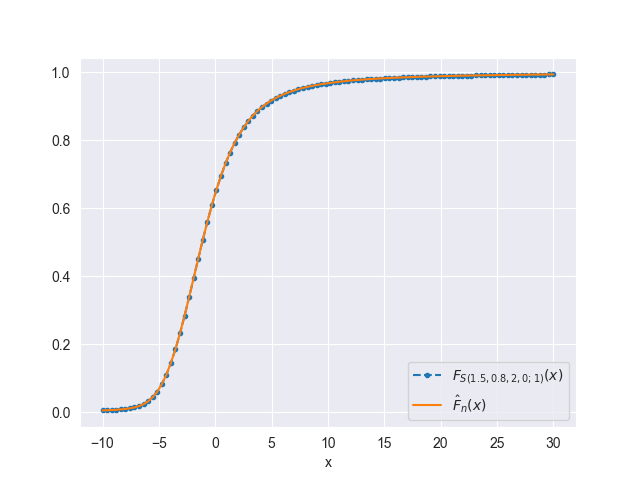
\includegraphics[width=1\linewidth]{images/stable_CDF.png}
				\caption{C}
			\end{subfigure}
			\begin{subfigure}[r]{.5\textwidth}
				\centering
				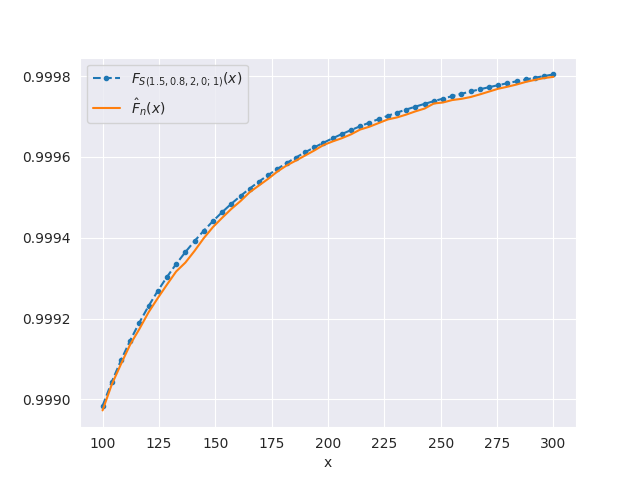
\includegraphics[width=1\linewidth]{images/stable_CDF_large_x.png}
				\caption{B}
			\end{subfigure}
			\caption{A}
		\end{figure}

		\begin{figure}
			\centering
			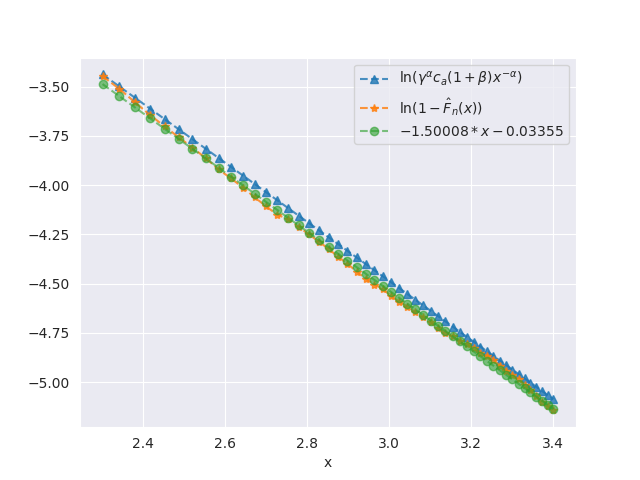
\includegraphics[width=1\linewidth]{images/compare_cdf_plots_type_1.png}
			\caption{C}
		\end{figure}

		\begin{figure}
			\begin{subfigure}{.5\textwidth}
				\centering
				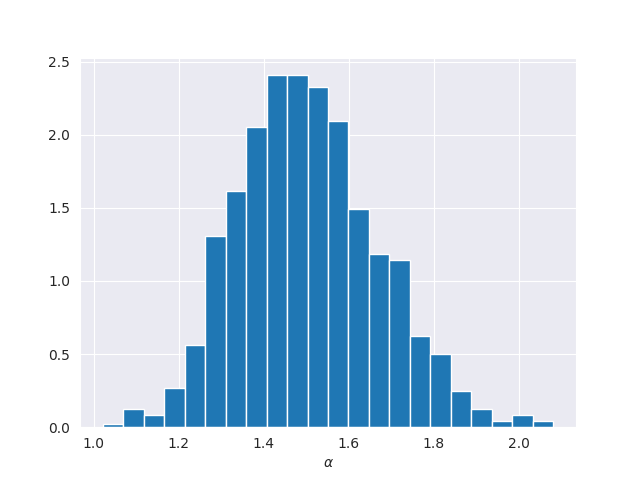
\includegraphics[width=1\linewidth]{images/cdf_alpha_hist.png}
				\caption{C}
			\end{subfigure}
			\begin{subfigure}[r]{.5\textwidth}
				\centering
				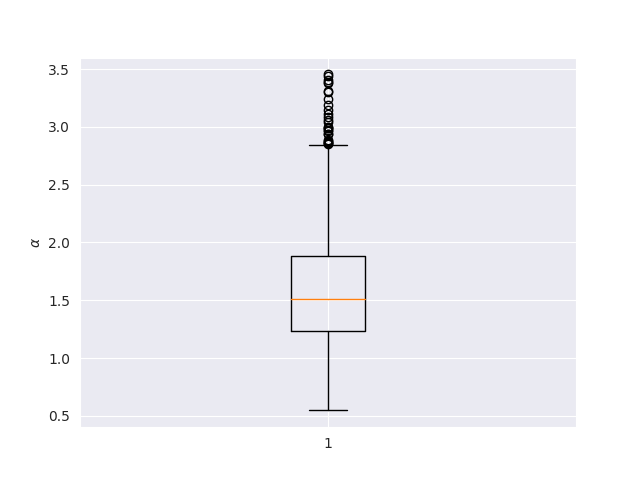
\includegraphics[width=1\linewidth]{images/cdf_alpha_boxplot.png}
				\caption{B}
			\end{subfigure}
			\caption{A}
		\end{figure}

\end{document}